The main goal of the \tauhadvis reconstruction employed at the ATLAS
experiment is to reconstruct \tauhadvis candidates that originate from
hadronic decays of \tauleptons (\truetauhadvis) with high
efficiency. As a result of this approach, objects from sources other
than \tauhad are frequently reconstructed as \tauhadvis candidates
(\faketauhadvis). Tau identification aims to distinguish between
\tauhadvis candidates from \tauhad and other sources.

The primary source of \faketauhadvis are quark- or gluon-initiated
jets due to the purely hadronic and jet-like signature of \tauhadvis
at the ATLAS experiment. Electrons can be another, less abundant,
source of \faketauhadvis which have to be distinguished from
\truetauhadvis using a dedicated algorithm. In the following, the
former classification task is referred to as \tauid while the latter
is referred to as \emph{electron veto}. Consequently, this chapter is
concerned with classifying the origin of \tauhadvis candidates as
either originating from \tauhad or from quark- or gluon-initiated
jets.

A number of features can be exploited to distinguish between
\tauhadvis candidates originating from \tauhad and quark- or
gluon-initiated jets:
\begin{description}

\item[\taulepton mass] The \taulepton has a mass of
  \SI{1.777}{\GeV}~\cite{pdg2020} and is therefore sufficiently
  massive to decay hadronically while still having a small mass
  compared to the energy scales of processes studied at the ATLAS
  experiment.

  The \taulepton mass can be used directly as a feature by considering
  the invariant mass of the reconstructed secondary particles
  associated to a \tauhadvis candidate. Ignoring reconstruction
  effects, the invariant mass of the visible decay products of \tauhad
  is bounded by the \taulepton mass. This is not the case for
  \tauhadvis candidates originating from quark- or gluon-initiated
  jets which do not have a strict bound.

  The other features, described hereafter, are consequences of, or
  closely related to the mass of the \taulepton.

\item[Particle multiplicity] Hadronic decays of \tauleptons produce
  few (visible) daughter particles. Most decays produce one or three
  charged hadrons (most frequently $\pi^{\pm}$) and zero to two
  neutral pions.
  % Ellis, Stirling, Webber: 6.4 Quark and gluon jet differences
  In contrast, the average multiplicity of charged and neutral
  particles inside of jets originating from the fragmentation of
  partons produced in hard scattering interactions is large and
  increases with the momentum of the
  jet~\cite{Ellis:1996mzs,STDM-2015-12}. Therefore, requirements on
  (charged) particle multiplicties are effective at rejecting
  \tauhadvis candidates originating from quark- or gluon-initiated
  jets.\footnote{Gluon-initiated jets have, on average, a larger
    particle multiplicity and a broader angular distribution of
    particles compared to quark-initiated jets due to the larger
    effective colour charge of
    gluons~\cite{Ellis:1996mzs}. Consequently, quark-initiated jets
    are more likely to be reconstructed and identified as \tauhadvis
    candidates.}

\item[Collimated daughter particles] Analyses typically consider
  \tauhadvis candidates with transverse momenta exceeding
  \SI{20}{\GeV}. At these momentum scales the decay products of
  \tauleptons are collimated due to the Lorentz boost of the lepton,
  leading to the characteristic signature of a narrow jet with few
  visible particles. Requirements on the isolation of \tauhadvis
  candidates allow to reject candidates originating from quark- or
  gluon-initiated jets which have wider angular distribution of
  hadrons.

\item[Lifetime]

\end{description}

(Recurrent) neural network-based method:
- Previously boosted decision tree using high-level variables
- Using neural networks to combine high-level information with
low-level information in the form of sequences of tracks and clusters
associated to \tauhadvis candidates.

The identification method is a continuation of the method proposed in
Ref.~\cite{cdeutsch-master} and was published as
Ref.~\cite{ATL-PHYS-PUB-2019-033} with the ATLAS collaboration.








BDT approach and input variables

Motivated by RNNIP: \cite{ATL-PHYS-PUB-2017-003}



The method described in this chapter is adopted by the ATLAS
collaboration as the recommended \tauid algorithm for analyses using
the \SI{139}{\per\femto\barn} $pp$-collision dataset recorded with the
ATLAS detector during Run~2 of the LHC.

Sections???


\todo[inline]{Mention somewhere what the differences between quark and
  gluon jets are.}


\section{Simulated Event Samples}

The studies presented in this chapter

Training setup, i.e.\ samples (dijet \& $\gamma^*$)

Use as source of \tauhadvis candidates.

Tauhad Truth matching???

Reweighting of (fake) \tauhad \pT


\section{Tau Reconstruction and Identification}


\subsection{Seed Jet}

Seeded with AntiKt 0.4 jets on TopoClusters at the LC scale.


\subsection{Tau Vertex Association}

TJVA


\subsection{Track Association}

\cite{duschinger}


\subsection{Energy Calibration}

MVA TES


\subsection{Electron Veto}

\subsection{Tau Identification}



\section{Tau Identification with Recurrent Neural Networks}

\subsection{Input Variables}

\begin{table}[htbp]
  \centering

  \caption{Input variables. Adopted from
    Ref.~\cite{ATL-PHYS-PUB-2019-033}.}%
  \label{tab:tauid_input_variables}

  \renewcommand{\arraystretch}{1.2}

\begin{tabular}{clccp{10.5cm}}
  \toprule
  & Observable & 1-prong & 3-prong & Description \\
  \midrule
  \parbox[t]{2mm}{\multirow{11}{*}{\rotatebox[origin=c]{90}{High-level inputs}}}
  & $p_\text{T}$ & \checkmark & \checkmark
  & Calorimeter-based estimate of \tauhadvis candidate \pT. \\

  & $f_\text{cent}$                & \checkmark & \checkmark
  & Ratio of \ET deposited in calorimeter cells (at EM scale) in cones of $\Delta R < 0.1$ and $\Delta R < 0.2$ about the \tauhadvis axis. \\

  & $f_\text{leadtrack}^{-1}$      & \checkmark & \checkmark
  & Ratio of \ET deposited in calorimeter cells (at EM scale) in a cone of $\Delta R < 0.2$ about the \tauhadvis axis and the \pT of the \pT-leading \emph{core} track. \\

  & $\Delta R_\text{max}$          & \checkmark & \checkmark
  & Maximum $\Delta R$ between core tracks and the \tauhadvis axis. \\

  & $|S_\text{leadtrack}|$         & \checkmark &
  & Transverse impact parameter significance of the \pT-leading track. \\

  & $S_\text{T}^\text{flight}$     &           & \checkmark
  & Transverse flight path significance. \\

  & $f_\text{iso}^\text{track}$    & \checkmark & \checkmark
  & Ratio of scalar sum of \pT of \emph{isolation} tracks and scalar sum of \pT of \emph{core} and \emph{isolation} tracks. \\

  & $f_\text{track}^\text{EM}$     & \checkmark & \checkmark
  & Ratio of the energy in EM clusters$^\dagger$ and the scalar sum of momenta of \emph{core} tracks. \\

  & $p_\text{T}^\text{EM+track}/\pT$ & \checkmark & \checkmark
  & \pT of the \tauhadvis estimated from the momenta of \emph{core} tracks and the two most energetic EM clusters$^\dagger$ divided by the \pT of the calorimetric measurement. \\

  & $m^\text{EM+track}$            & \checkmark & \checkmark
  & Invariant mass of the system of \emph{core} tracks and the two most energetic EM clusters$^\dagger$. \\

  & $m^\text{track}$               &           & \checkmark
  & Invariant mass of the system of \emph{core} tracks. \\
  \midrule
  \parbox[t]{2mm}{\multirow{9}{*}{\rotatebox[origin=c]{90}{Track inputs}}}
  & $p_\text{T}^\text{seed jet}$ & \checkmark & \checkmark
  & \pT of the jet seeding the \tauhadvis candidate. \\

  & $p_\text{T}^\text{track}$    & \checkmark & \checkmark
  & \pT of the track. \\

  & $\Delta\eta^\text{track}$    & \checkmark & \checkmark
  & Difference in $\eta$ between track and \tauhadvis axis. \\

  & $\Delta\phi^\text{track}$    & \checkmark & \checkmark
  & Angle between track and \tauhadvis axis in the transverse plane. \\

  & $|d_0^\text{track}|$         & \checkmark & \checkmark
  & Absolute value of the transverse track impact parameter. \\

  & $|z_0^\text{track} \sin\theta|$ & \checkmark & \checkmark
  & Absolute value of the product of longitudinal track impact parameter and sine of the polar angle of the track. \\

  & $N_\text{IBL hits}$   & \checkmark & \checkmark
  & Number of hits on the track in the IBL. \\

  & $N_\text{Pixel hits}$ & \checkmark & \checkmark
  & Number of hits on the track in pixel detector layers. \\

  & $N_\text{SCT hits}$   & \checkmark & \checkmark
  & Number of hits on the track in SCT layers. \\

  \midrule
  \parbox[t]{2mm}{\multirow{7}{*}{\rotatebox[origin=c]{90}{Cluster inputs}}}
  & $p_\text{T}^\text{jet seed}$ & \checkmark & \checkmark
  & \pT of the jet seeding the \tauhadvis candidate. \\

  & $E_\text{T}^\text{cluster}$ & \checkmark & \checkmark
  & \ET of the cluster. \\

  & $\Delta\eta^\text{cluster}$      & \checkmark & \checkmark
  & Difference in $\eta$ between cluster and \tauhadvis axis. \\

  & $\Delta\phi^\text{cluster}$      & \checkmark & \checkmark
  & Angle between cluster and \tauhadvis axis in the transverse plane. \\

  & $\lambda_\mathrm{cluster}$             & \checkmark & \checkmark
  & Longitudinal distance of the cluster barycentre from the calorimeter front face. \\

  & $\langle \lambda_\mathrm{cluster}^2\rangle$ & \checkmark & \checkmark
  & Second longitudinal cluster moment. \\

  & $\langle r_\mathrm{cluster}^2\rangle$             & \checkmark & \checkmark
  & Second radial cluster moment. \\
  \bottomrule
\end{tabular}

%%% Local Variables:
%%% mode: latex
%%% TeX-master: "../phd_thesis"
%%% End:

\end{table}

Plots of high-level variables

Plots of (some) low-level variables???


\subsection{Network Architecture}

\begin{figure}[htbp]
  \centering

  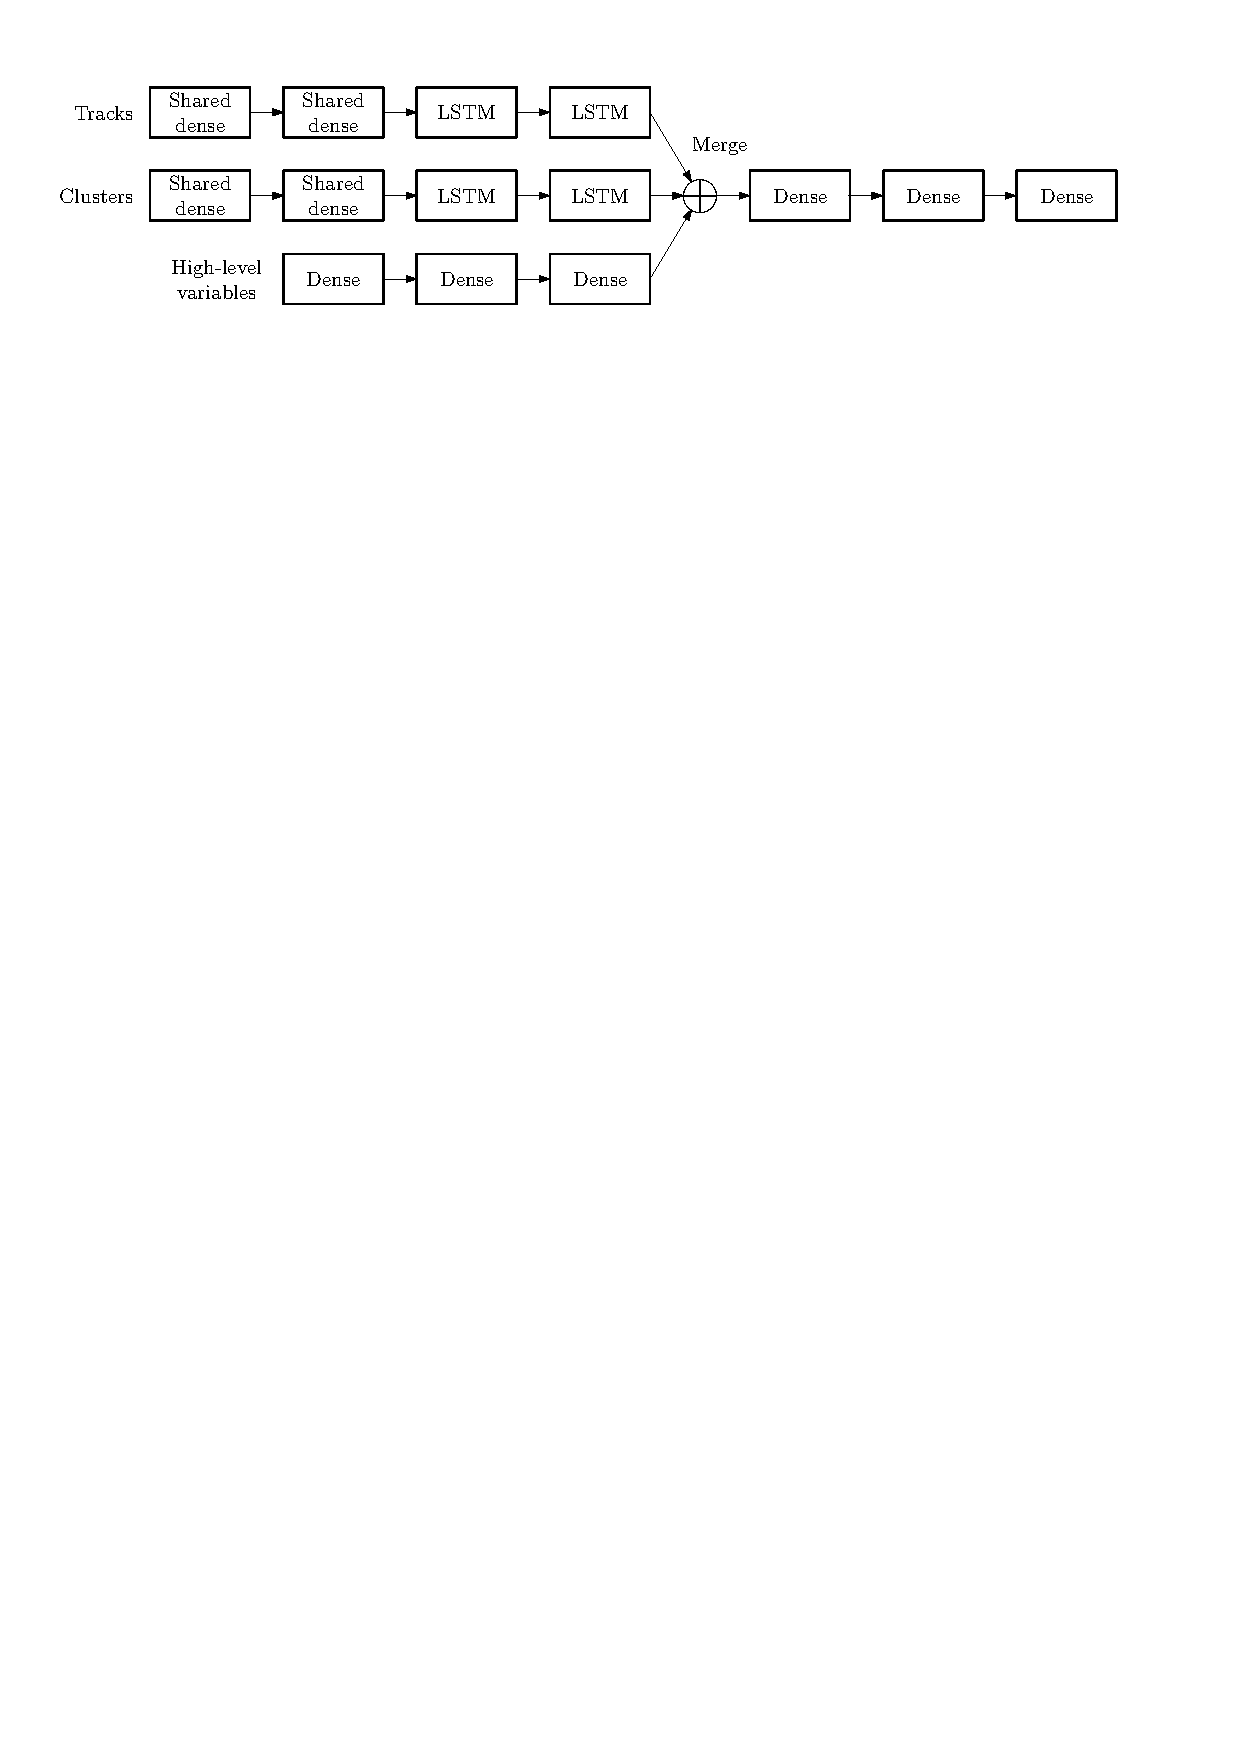
\includegraphics[width=0.95\textwidth]{tauid/pubnote/rnn_network_architecture}

  \caption{Network Architecture of the RNN \tauhad-identification
    algorithm \cite{ATL-PHYS-PUB-2019-033}}
  \label{fig:tauid_network_architecture}
\end{figure}

\subsection{Training and evaluation}

Keras Tensorflow lwtnn \cite{lwtnn,keras,tensorflow2015-whitepaper,lstm}

Used in the software suite
\textsc{Athena}~\cite{ATL-SOFT-PUB-2021-001}.

\subsection{Working Point Definition}


\subsection{Calibration}


\section{Tau Identification Performance}

\begin{figure}[htbp]
  \centering

  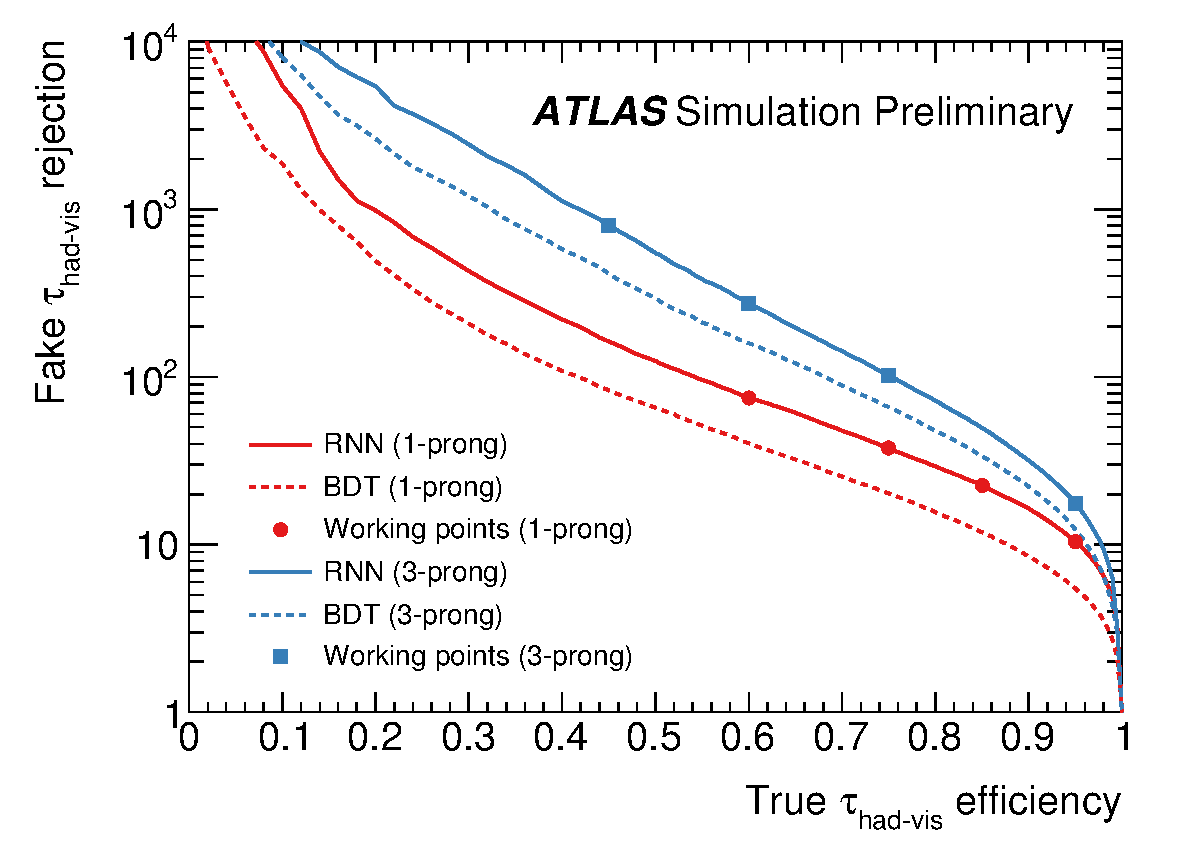
\includegraphics[width=0.6\textwidth]{tauid/pubnote/rnn_bdt_roc}

  \caption{Receiver operating characteristic of the RNN
    \tauhad-identification algorithm \cite{ATL-PHYS-PUB-2019-033}}
  \label{fig:tauid_rnn_bdt_roc_comparison}
\end{figure}


\begin{table}
  \centering

  \caption{List of defined working points with fixed true \tauhadvis
    selection efficiencies and the corresponding background rejection
    factors for misidentified \tauhadvis in dijet events for the BDT
    and RNN classifiers. Adapted from~\cite{ATL-PHYS-PUB-2019-033}.}%
  \label{tab:rnn_wps}

  \begin{tabular}{lcccccc}
    \toprule
                  & \multicolumn{2}{c}{Signal efficiency} & \multicolumn{2}{c}{Background rejection (BDT)} & \multicolumn{2}{c}{Background rejection (RNN)} \\
    Working point  & 1-prong & 3-prong & 1-prong & 3-prong & 1-prong & 3-prong \\
    \midrule
    Tight          & 60\%    & 45\%    & 40      & 400  & 70   & 700 \\
    Medium         & 75\%    & 60\%    & 20      & 150  & 35   & 240 \\
    Loose          & 85\%    & 75\%    & 12      & 61   & 21   & 90  \\
    Very loose     & 95\%    & 95\%    & 5.3     & 11.2 & 9.9  & 16  \\
    \bottomrule
  \end{tabular}
\end{table}

\subsection{Use at the HLT?}

\cite{ATL-DAQ-PUB-2019-001}


\section{Conclusion and Outlook}


To be replaced by ``deep sets'' (permutation invariance). Based on the
same idea and same expected performance but significantly improved
training and prediction time.

%%% Local Variables:
%%% mode: latex
%%% TeX-master: "../../phd_thesis"
%%% End:
